\chapter{Proposed Method}
\label{chap:Method}
In this chapter, each part of the proposed method is described in detail.

\section{Overview}
The proposed method consists of three modules: input features, text-to-speech module, and talking head generation module.
The input features are the input of the text-to-speech module. The text-to-speech module is the input of the talking head generation module.
The talking head generation module is the output of the proposed method.
The overview of the proposed method is shown in Figure \ref{fig:overview}. Encodec refers to the encoder of Encodec, while Decodec refers to the decoder of Encodec.
The main contribution of this paper is the yellow-highlighted audio token processor part and the face landmark loss, which maintains a constant face size. This will be explained further below.
\begin{figure}
    \centering
    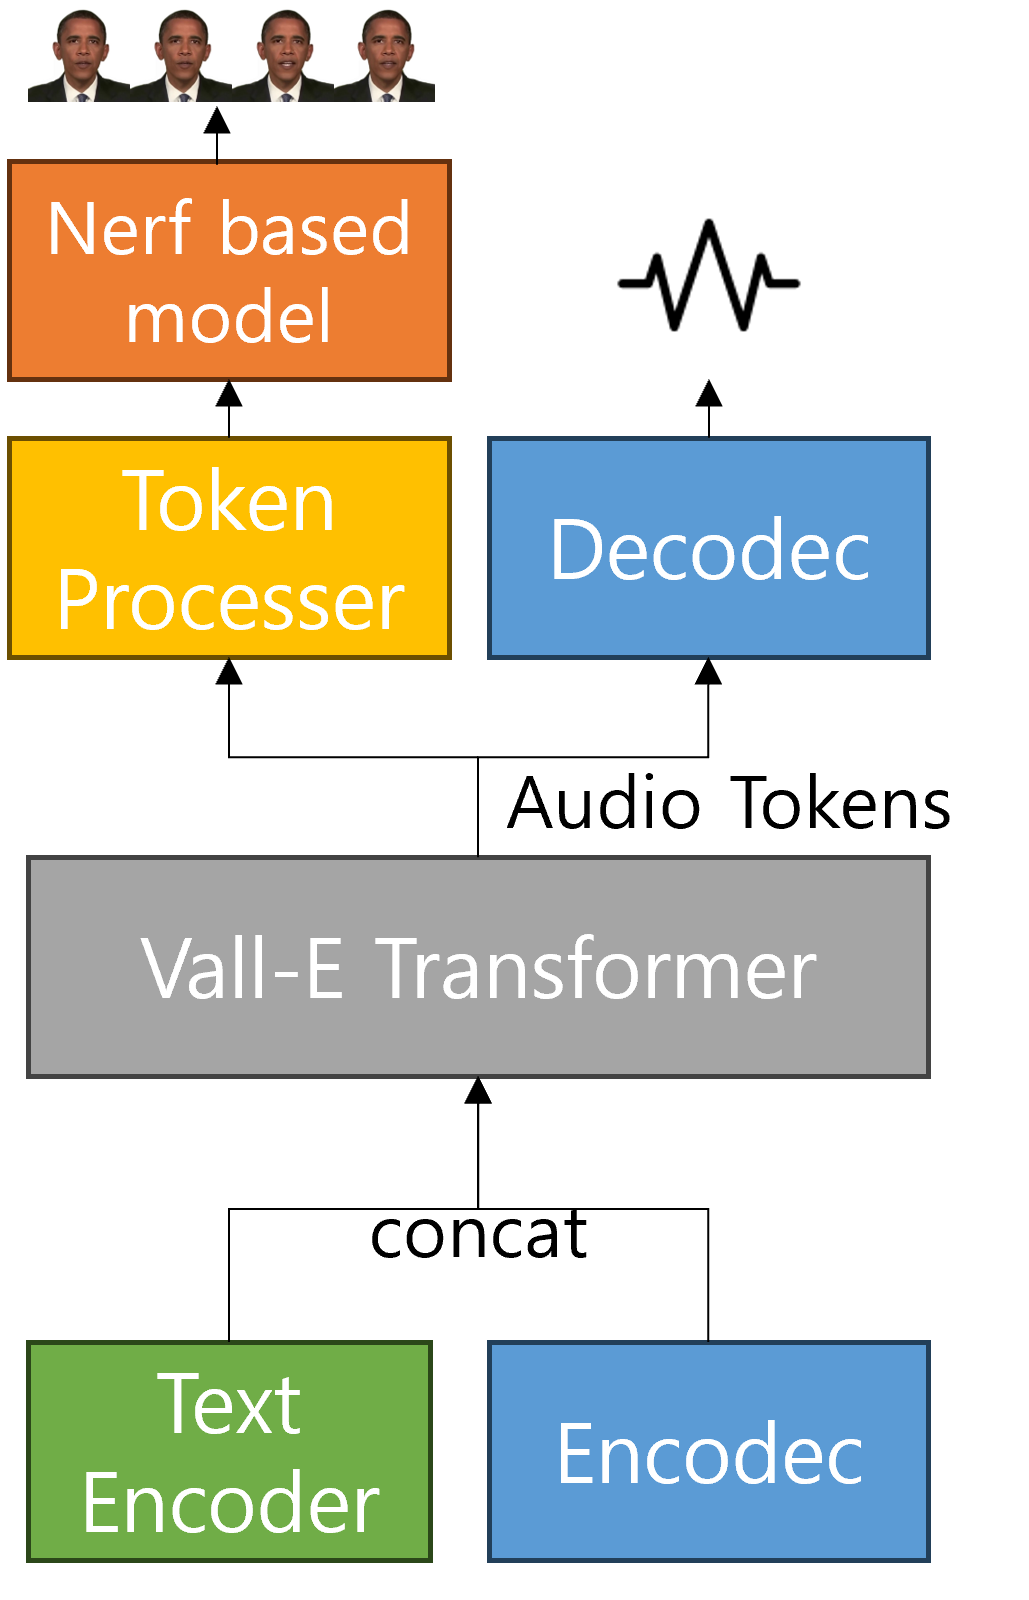
\includegraphics[width=0.8\textwidth]{figures/figure_chap_3/overview.png}
    \caption{Overview of the proposed method}
    \label{fig:overview}
\end{figure}
\section{input features}
\subsection{audio and text features}
\label{sec:audio_and_text_features}
The input features are the input of the text-to-speech module.
Input audio resampled to 24kHz and encoded by the encodec\cite{EnCodec}.
EnCodec is trained on the DNS Challenge 4, common voice and audioset.
The tokens extracted from the EnCodec are processed discribed at \ref{fig:feature}.
As illustrated in the figure, the same order of token values from consecutive 3 tokens were concatenated,
since the output of the same residual vector quantizer in consecutive tokens tends to have similar values.
The reason for concatenating tokens in groups of three is three tokens being generated for every 25ms.
This is the same as the frame rate of the video feature sequence chunk size.
And the tokens are grouped into window size of 16 for smoothing.

\begin{figure}
    \centering
    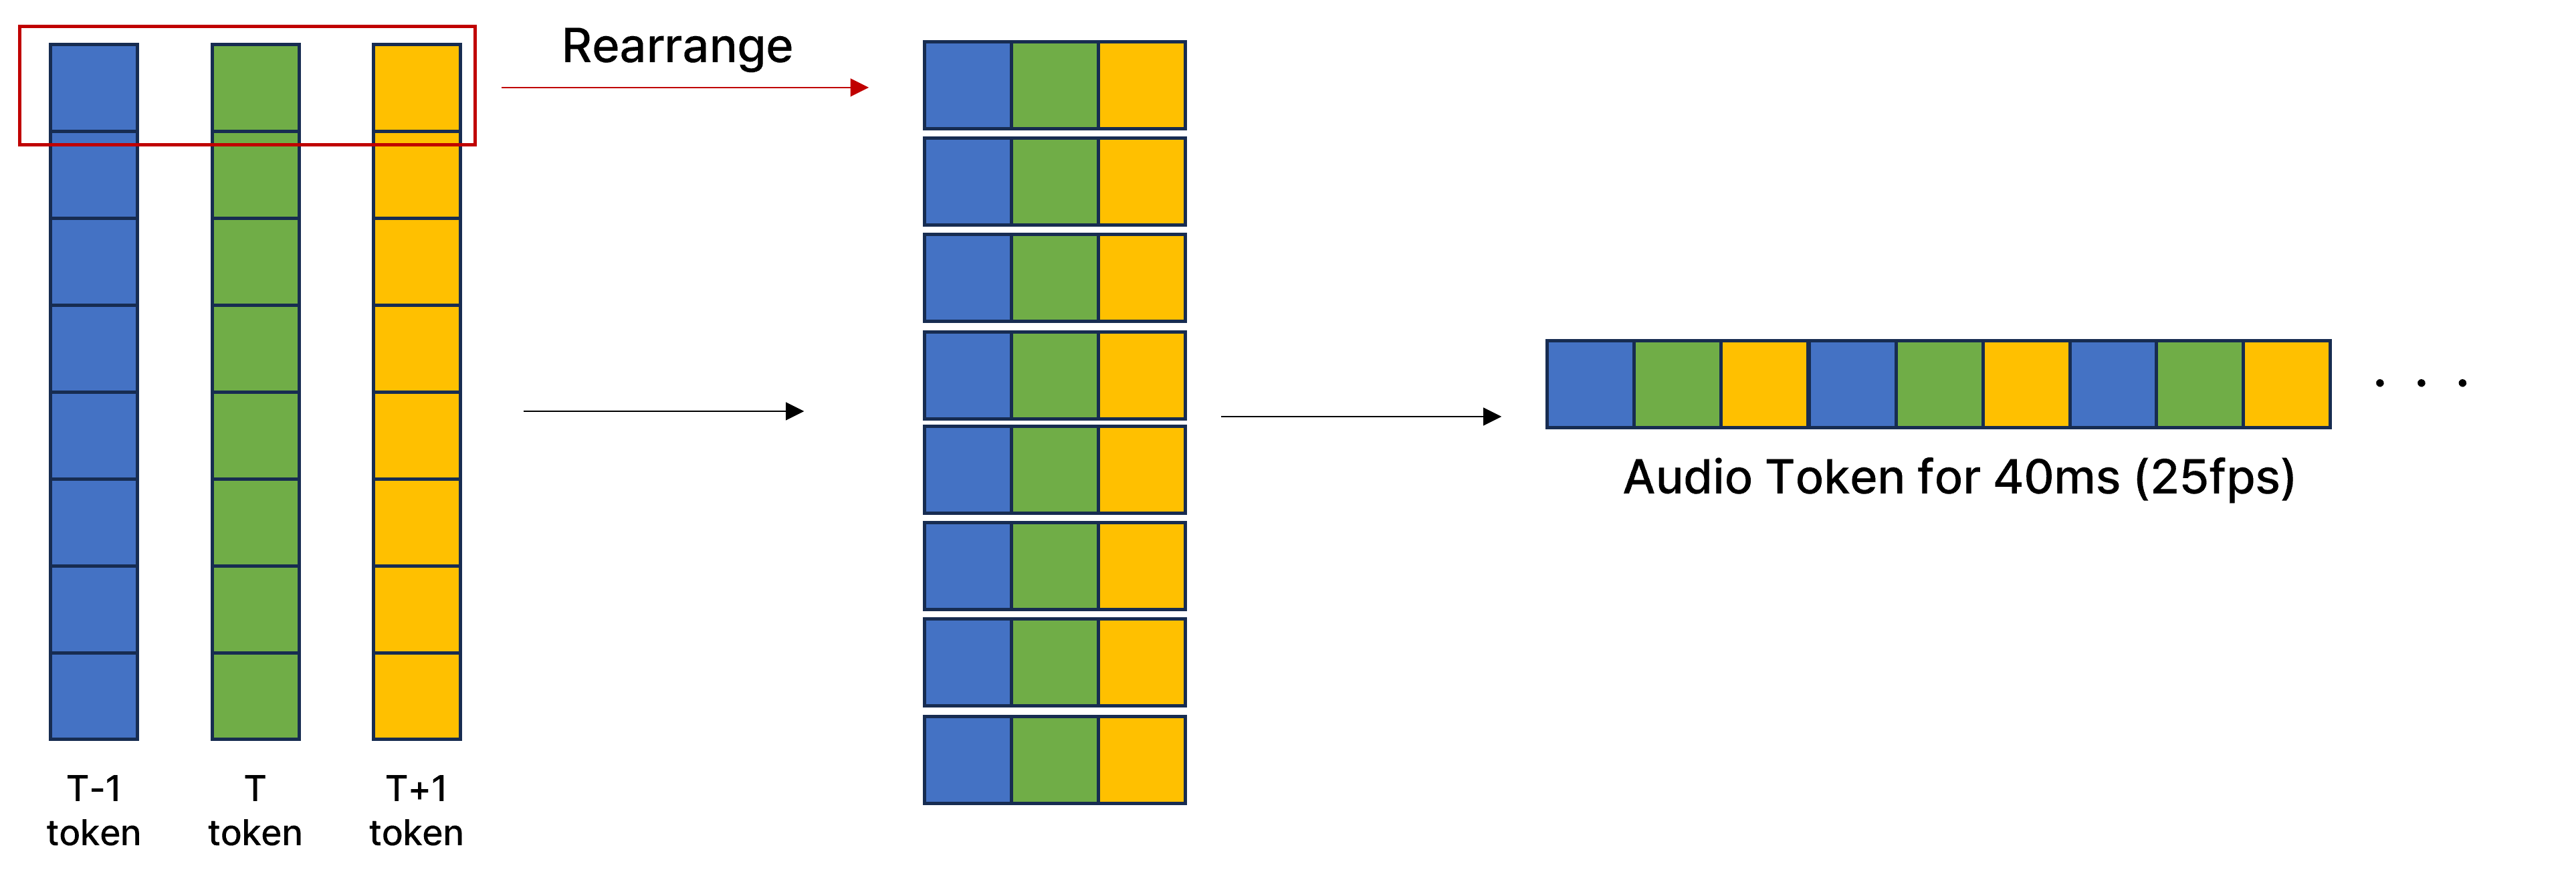
\includegraphics[width=0.8\textwidth]{figures/figure_chap_3/feature.png}
    \caption{EnCodec feature processing}
    \label{fig:feature}
\end{figure}
 

\subsection{video features}
Video features are the input of the talking head generation module, when the talking head generation module is trained.
Additionally, face landmark extracted four the speaker's eye-movement and lip movement naturalness.



\section{Text-to-Speech Module}
Text-to-speech module generates the audio feature of the speaker's voices.
In this study, TTS model is Vall-E-X, trained with Librispeech and LibriTTS.
Encodec compression option is same as audio encoder in \ref{sec:audio_and_text_features}.

\section{NeRF-based Talking Head Generation Module}
Talking head generation module generates the talking head video of the speaker.
In this study, Rad-NeRF\cite{tang2022radnerf} picked for the talking head generation module baseline.
The audio feature extraction module is modifeid to better fit the proposed method.
Batch-normalization is added to the front of the audio feature extraction module.
Since the EnCodec feature has a value range between 0 and 1024,
This range could be a result of the encoding process or a design choice to standardize the feature values,
making them suitable for subsequent processing steps that might require normalized or bounded input values.
after the batch-normalization, the audio processing module is similar as the original Rad-NeRF.
\begin{figure}
    \centering
    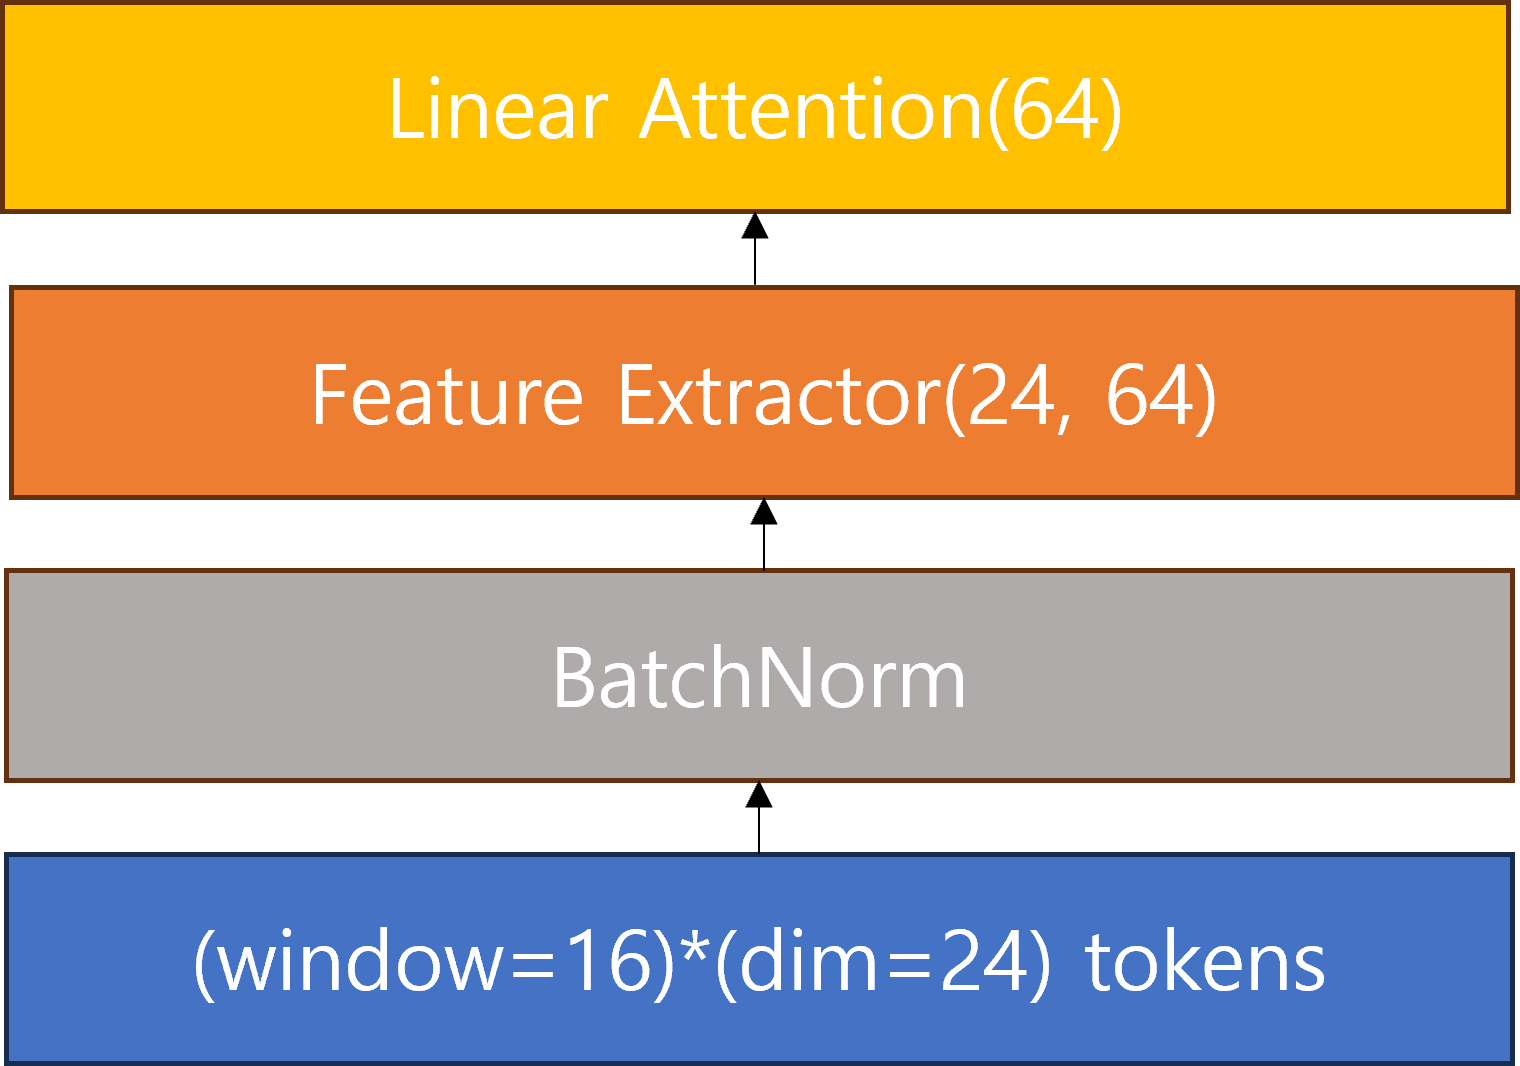
\includegraphics[width=0.4\textwidth]{figures/figure_chap_3/afp.png}
    \caption{audio feature extraction module}
    \label{fig:afp}
\end{figure}

\section{Loss Function}
In addressing the challenge of inconsistent head proportions in dynamic facial imagery within Neural Radiance Fields (NeRF) based models, a novel approach is proposed. Traditional NeRF implementations, which primarily utilize Mean Squared Error (MSE) loss against original images, often result in fluctuating head sizes in generated sequences. This issue is particularly pronounced in sequences involving speech or facial movements.
To mitigate this, an enhanced loss function is introduced, integrating a face landmark loss with the standard MSE loss. This additional component aims to stabilize and normalize head dimensions in synthesized images, addressing the inconsistencies arising from the use of MSE loss alone.
The proposed loss function is defined as follows:
\begin{equation}
    \mathcal{L} = \mathcal{L}_{MSE} + \lambda \mathcal{L}_{landmark}
\end{equation}
where $\mathcal{L}_{MSE}$ is the MSE loss, $\mathcal{L}_{landmark}$ is the face landmark loss, and $\lambda$ is the weight of the face landmark loss.
The face landmark loss is defined as follows:
\begin{equation}
    \mathcal{L}_{landmark} = \frac{1}{N}\sum_{i=1}^{N}||\mathbf{p}_i - \mathbf{p}_i^*||_2
\end{equation}
where $\mathbf{p}_i$ is the predicted face landmark, $\mathbf{p}_i^*$ is the ground truth face landmark, and $N$ is the number of face landmarks.
The face landmark loss is calculated using the normalized MSE loss between the predicted face landmarks and the ground truth face landmarks.
